\documentclass[10pt]{book}
\usepackage{graphicx}
\usepackage{subfig} % make it possible to include more than one captioned figure/table in a single float
\usepackage[utf8]{inputenc}
\usepackage{hyperref}
\usepackage[intlimits]{amsmath}
\usepackage{amssymb}
\setlength{\oddsidemargin}{15.5pt} 
\setlength{\evensidemargin}{15.5pt}
\pretolerance=2000
\tolerance=3000
\renewcommand{\figurename}{Figura}
\renewcommand{\chaptername}{Cap\'{i}tulo}
\renewcommand{\contentsname}{\'{I}ndice}
\renewcommand{\tablename}{Tabla}
\renewcommand{\bibname}{Bibliograf\'{i}a}
\renewcommand{\appendixname}{Ap\'endices}


\usepackage{geometry}
 \geometry{
 a4paper,
 left=15mm,
 right=10mm,
 top=20mm,
 bottom=20mm,
 }

\begin{document}

\paragraph 1a) 
\begin{figure}[!ht]
 \centering
 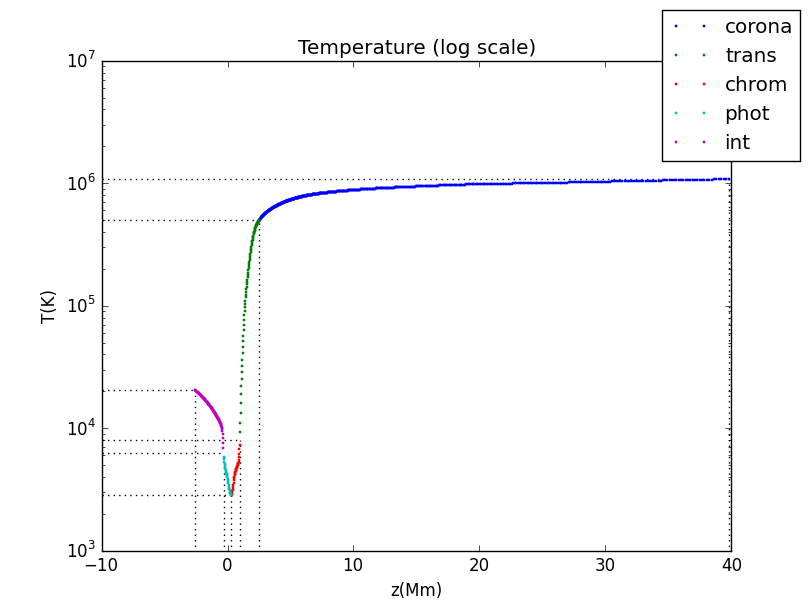
\includegraphics[scale=0.5]{tempLayers.png}
 \caption{\emph{Temperature vs z plot. logarithmic y scale}}
\end{figure}


Temperature layers (from top to bottom), interval of temperatures measured in K and code conditions  from: 
\url{http://www.nasa.gov/mission_pages/iris/multimedia/layerzoo.html}

\begin{description}

\item corona between [39.802200, 2.535930] Mm temperatures: [1.080180e+06, 5.025160e+05] K ($\ge 500000$)
\item transition region between [2.516350, 0.991115] Mm temperatures: [4.991350e+05, 8.067640e+03] K  ($[50000, 8000)$)
\item chromosphere between [0.971556, 0.305708] Mm temperatures: [7.306160e+03, 2.843670e+03] K ($[8000, min(temperature)]$)
\item photosphere between [0.286093, -0.303487] Mm temperatures: [2.848470e+03, 6.297540e+03] K ($(min(temperature), 6500]$)
\item solar interior between [-0.323184, -2.592960] Mm temperatures: [6.837750e+03, 2.068340e+04] K ($ > 6500$)

\end{description}



\paragraph 1b)

$\mu = \frac{n_{H} + 4 n_{He}}{n_e + n_H + n_{He}} $

\begin{itemize}
\item totally ionized H and He $\implies n_e = n_H + 2 n_{He} \implies  \mu = \frac{n_{H} + 4 n_{He}}{2 n_H + 3 n_{He}} $

$n_H= 10 n_{He} \implies  \mu = \frac{14}{23}  = 0.6087$

\item neutral H and He $\implies n_e = 0 \implies  \mu = \frac{n_{H} + 4 n_{He}}{n_H + n_{He}} $

$n_H= 10 n_{He} \implies  \mu = \frac{14}{11}  = 1.2727$

\end{itemize}



\begin{figure}[!ht]
 \centering
 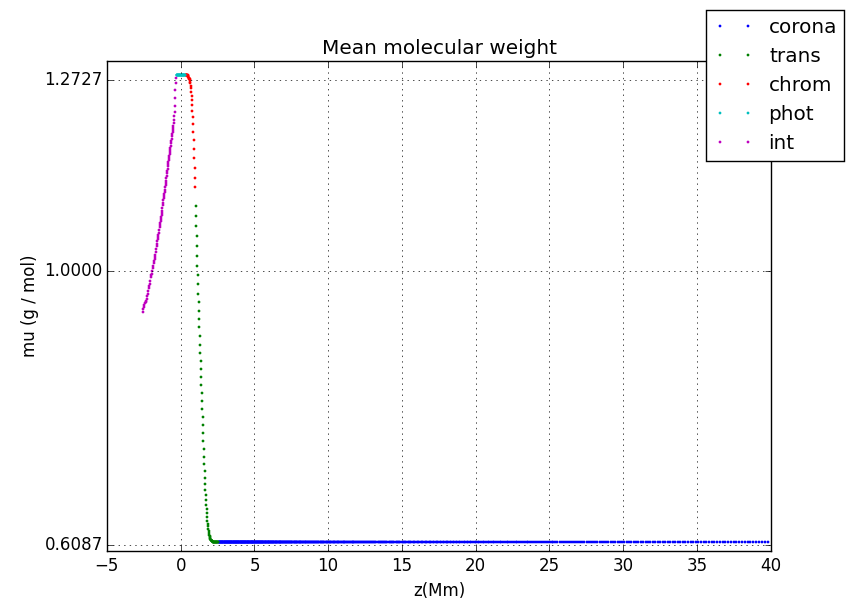
\includegraphics[scale=0.5]{mmmLayers.png}
 \caption{\emph{Mean molecular weight(g/mol) vs z plot} Upper limit close 1.2727 = $\mu$ in the case of neutral H and He, lower limit close to 0.6087 = $\mu$ calculated in the case of completely ionized H and He }
\end{figure}

$n_{He}  = \frac{1}{10} n_H \implies \mu = \frac{n_{H} + \frac{4}{10} n_{H}}{n_e + n_H +\frac{1}{10} n_{H}} $
  
$\implies \mu (1 + \frac{11}{10} \frac{n_{H}}{n_e})=  \frac{14}{10} \frac{n_{H}}{n_e}    $

$\implies \frac{n_H}{n_e} =  \frac{\mu}{1.4 - 1.1 \mu }   $


 

\begin{figure}[!ht]
 \centering
 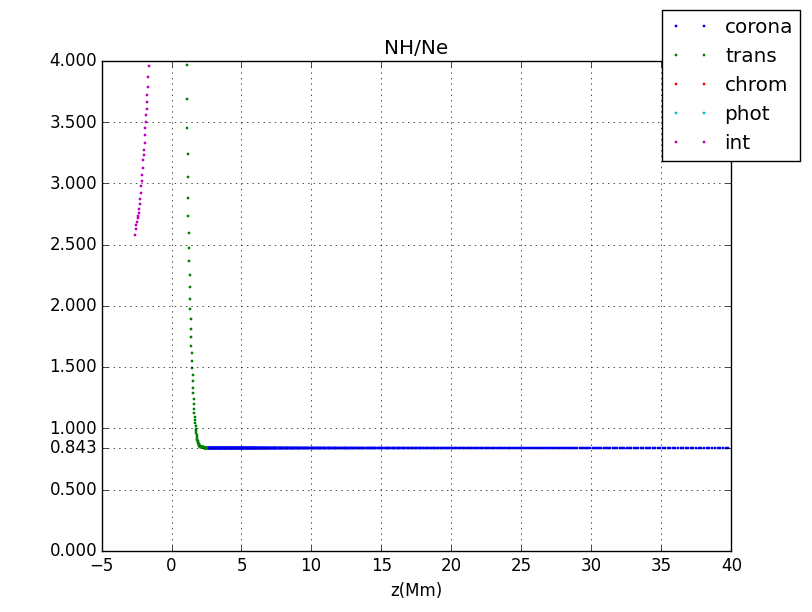
\includegraphics[scale=0.5]{nHDivNe.png}
 \caption{number of atoms of H / number of electrons }
\end{figure}

In the graphic(data from file) we can see the constant value in the corona of $\frac{n_H}{n_e} = 0.843 \approx = \frac{5}{6}$ 
which is the value we calculate in the case of totally ionized H and He and we expect this

\begin{figure}[!ht]
 \centering
 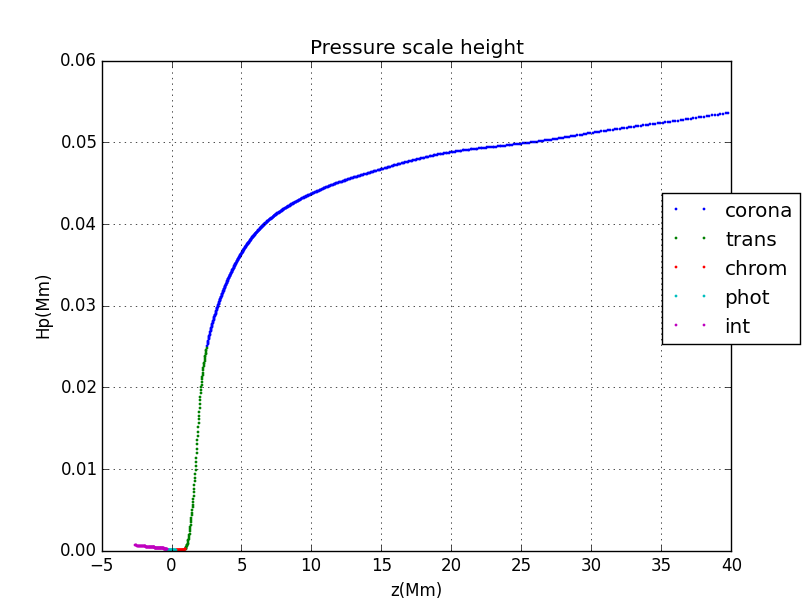
\includegraphics[scale=0.5]{hpLayers.png}
 \caption{Pressure scale height}
\end{figure}




\begin{figure}[!ht]
 \centering
 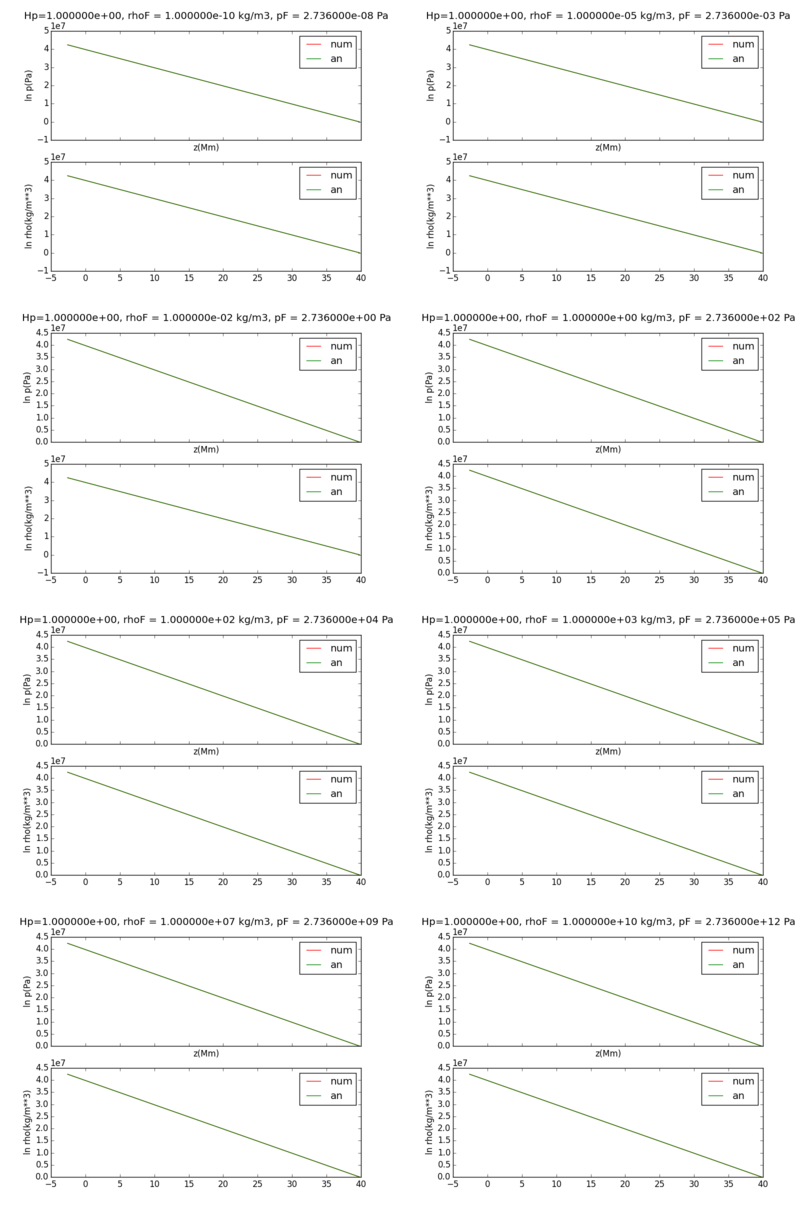
\includegraphics[scale=0.5]{allanalytic.png}
 \caption{Analytic test}
\end{figure}

\begin{figure}[!ht]
 \centering
 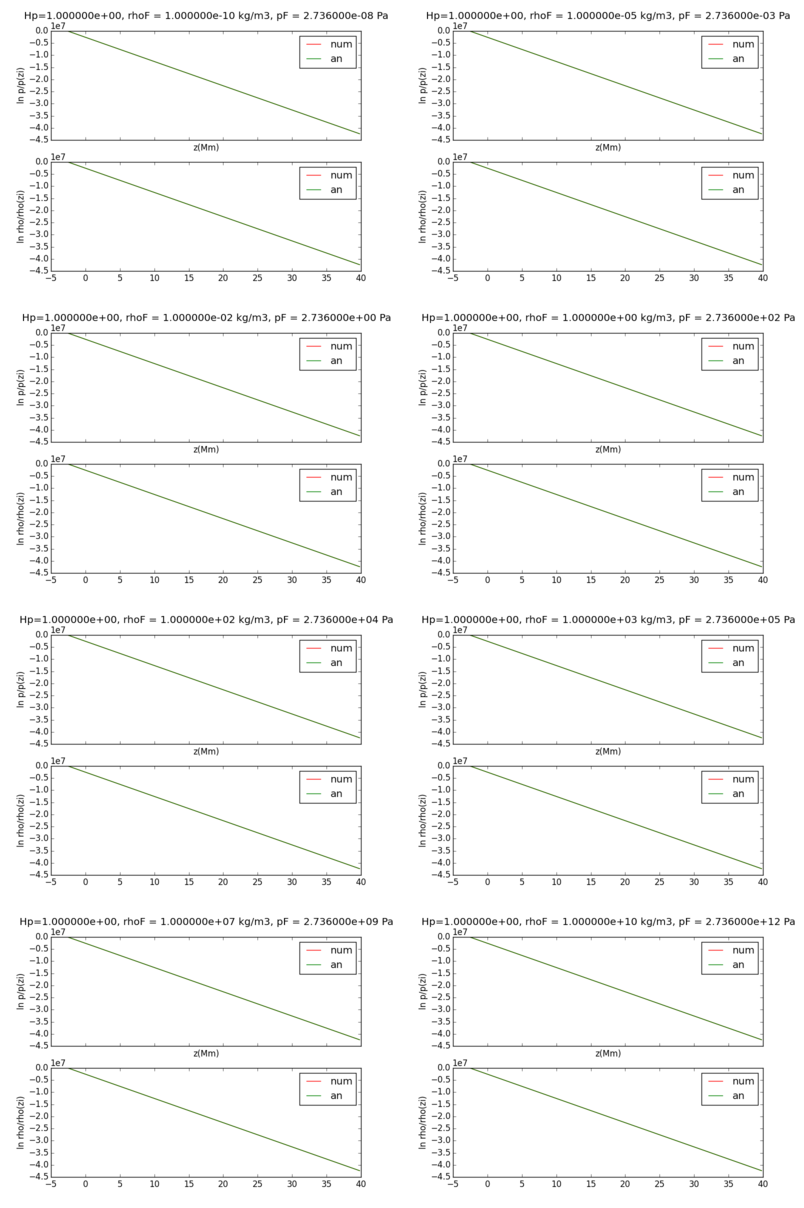
\includegraphics[scale=0.5]{allanalytic2.png}
 \caption{Analytic test}
\end{figure}


\begin{figure}[!ht]
 \centering
 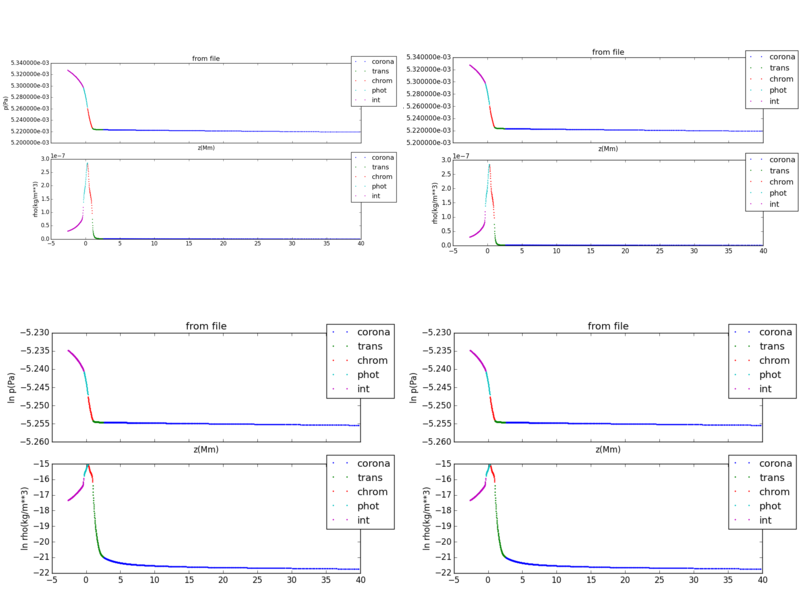
\includegraphics[scale=0.5]{allfile.png}
 \caption{top pres and density, bottom ln (pres) and ln (density), left outward - inward integration, right inward - outward integration}
\end{figure}





\end{document}
